\documentclass [titlepage,12pt,letter] {article}
\pagestyle{myheadings}


\usepackage{graphicx} 
\usepackage{epsfig}
\usepackage{subfigure}
\usepackage{fancyhdr}
\usepackage{url} 
\usepackage{amsmath}
\usepackage{algorithm} 
\usepackage{algorithmic}
\pagestyle{fancy}



\fancyhead{}
\fancyfoot{}
			
\lhead{CSC349A Lecture Notes}
\rhead{Little, Rich}


\setcounter{page}{1}
\cfoot{\thepage}




\begin{document} 


These are the lecture notes for CSC349A Numerical Analysis taught by
Rich Little. They roughly correspond to
the material covered in each lecture in the classroom but the actual
classroom presentation might deviate significantly from them depending
on the flow of the course delivery. They are provided as a reference to
the instructor as well as supporting material for students who miss
the lectures. They are simply notes to support the lecture so the text
is not detailed and they are not thoroughly checked. Use at your own
risk. They are complimentary to the handouts. Many thanks to all the
guidance and materials I received from Dale Olesky who has taught this
course for many years and George Tzanetakis. 


\section{Numerical Integration (Quadrature)} 

{\bf Quadrature} - The process of determining areas e.g. area of a circle by inscribed
and superscribed polygons. This term is used to avoid confusion with
the numeric integration of differential equations.

Functions to be integrated or differentiated will typically be in one of three forms,

\begin{enumerate}
\item A simple continuous function - polynomial, exponential, trigonometric, etc.
\item A complicated continuous function that is difficult or impossible to differentiate/integrate analytically.
\item A tabulated, discrete function where we have a set of points $(x_i,f(x_i))$ - for example, sample data.
\end{enumerate}

We use numerical methods in all these cases. For 3, it is the only option. For 2, it may be the only choice or the most efficient choice. For 1, it is often the most efficient and simplest option. \\

\noindent 
{\bf Problem:} approximate the value of 
\[
\int_a^{b} f(x) dx
\] 
\noindent 
where $f(x)$ is such that it cannot be integrated analytically or it is known at only a finite set of points. 
\\
\noindent 
{\bf Procedure:} approximate $f(x)$ by an interpolating polynomial $P(x)$, and approximate $\int_{a}^{b} f(x)dx$ by $\int_a^{b} P(x)dx$
\\
Suppose $P_n(x)$ is the Lagrange form of the interpolating polynomial: 
\[
P_n(x) = \sum_{i=0}^{n} L_i(x) f(x_i)
\]
\noindent 
then 
\[
\int_{a}^{b} f(x)dx \approx \int_{a}^{b} \left [ \sum_{i=0}^{n} L_i(x) f(x_i) \right ] dx = \sum_{i=0}^{n} \left[ \int_a^b L_i(x) dx \right ] f(x_i) 
\]
\noindent 
which is of the form $\sum_{i=0}^{n} a_i f(x_i)$. 

Such an approximation is called a {\bf quadrature formula}, and $a_i$ are the {\bf quadrature coefficients} and $x_i$ are the {\bf quadrature points}, the points at which $f(x)$ is sampled to approximate $\int_{a}^{b} f(x)dx$. 

Types of quadrature formulas: 
\begin{itemize} 
\item Newton-Cotes closed - Sections 21.1 to 21.3 of the text.
\item Newton-Cotes open - Section 21.4.
\item Gaussian (omit) - In the text but we won't do.
\end{itemize} 

Any quadrature formula derived by integrating an interpolating polynomial at equally-spaced quadrature points is called a {\bf Newton-Cotes} formula. 

{\bf Gaussian formulas} obtain high accuracy by using optimally-chosen, unequally-spaced quadrature points. 

\subsection{Netwo-Cotes closed formulas} 

For any $n \geq 1$, subdivide [a,b] into $n$ subintervals of length 
$h = \frac{b-a}{n}$. 


\begin{figure} 
  \centering
  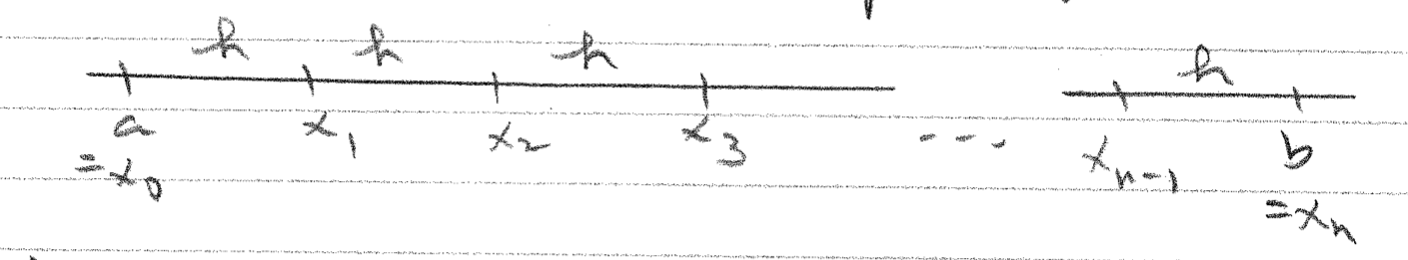
\includegraphics[scale=0.6]{linear_step_size}
  \label{fig:linear}
\end{figure}



Thus 
\begin{align*} 
x_{i+1} - x_{i} = h \\ 
x_i = x_0 + ih 
\end{align*} 

If $P_n(x)$ interpolates $f(x)$ at $a=x_0, x_1, x_2, \dots, b=x_n$ 
and 
\[
\int_{a}^{b} f(x)dx \approx \int_{a}^{b} P_n(x)dx 
\]
\noindent 
then the resulting quadrature formula is called a {\bf Newton-Cotes} closed formula. 


\subsection{Newton-Cotes closed quadrature formulas - n=1} 

The case $n=1$: 

\begin{figure} 
  \centering
  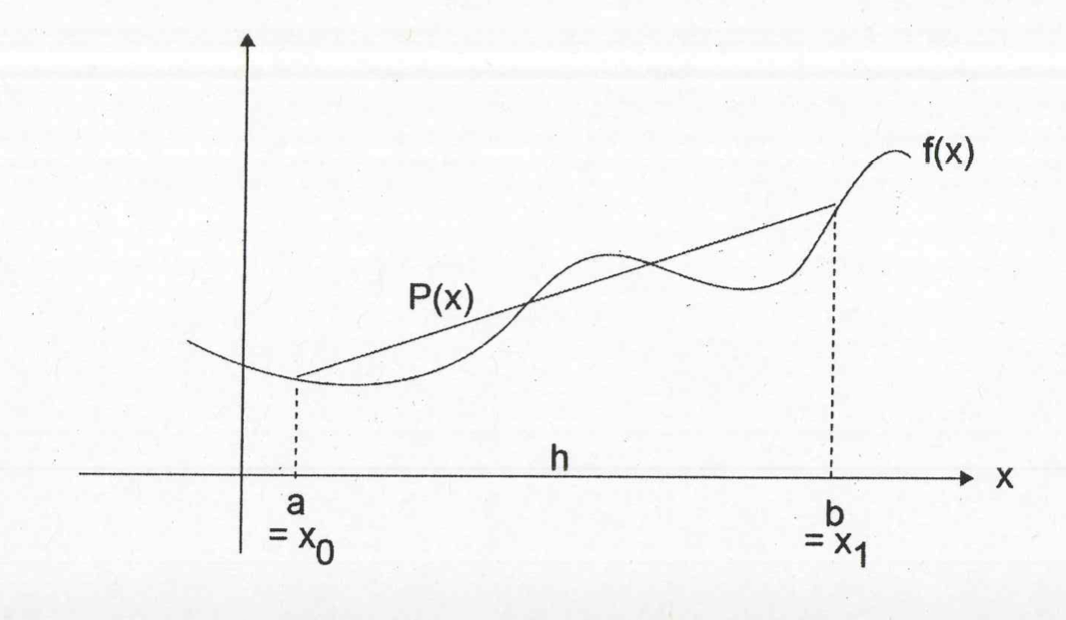
\includegraphics[scale=0.6]{linear_interpolating}
  \caption{Linear interpolating polynomial}
  \label{fig:linear}
\end{figure}
\noindent 
Here $h = b -a$. The (linear) interpolating polynomial is: 
\[
P(x) = \frac{x-x_1}{x_0-x_1}f(x_0) + \frac{x-x_0}{x_1-x_0} f(x_1) 
\]

The quadrature formula for approximating $\int_a^{b} f(x)dx$ is obtained by integrating P(x): 

\begin{align*} 
\int_{a}^{b} f(x)dx &\approx \int_{x_0}^{x_1} P(x)dx \\ 
   &= \left [ \int_{x_0}^{x_1} \frac{x-x_1}{x_0-x_1}f(x_0)dx \right ] + \left[ \int_{x_0}^{x_1} \frac{x-x_0}{x_1-x_0}f(x_1)dx \right ] \\
   &= \frac{f(x_0)}{x_0-x_1} \left [ \frac{x^2}{2} - x_1x \right ]_{x_0}^{x_1} + \frac{f(x_1)}{x_1-x_0} \left [ \frac{x^2}{2} - x_0x \right ]_{x_0}^{x_1} \\ 
   &= \frac{f(x_0)}{x_0-x_1} \left [ (\frac{x_1^2}{2} - x_1^2)- (\frac{x_0^2}{2} - x_1x_0)\right ] + \frac{f(x_1)}{x_1-x_0} \left [ (\frac{x_1^2}{2} - x_1x_0)- (\frac{x_0^2}{2} - x_0^2) \right ] \\ 
   &= \frac{f(x_0)}{x_0-x_1} \left [ -(\frac{x_1^2}{2} - x_1x_0 + \frac{x_0^2}{2}) \right ] + \frac{f(x_1)}{x_1-x_0} \left [ \frac{x_1^2}{2} - x_1x_0 + \frac{x_0^2}{2} \right ] \\ 
   &= \frac{f(x_0)}{2}\left [\frac{(x_1-x_0)^2}{(x_1-x_0)}\right ]+\frac{f(x_1)}{2}\left [\frac{(x_1-x_0)^2}{(x_1-x_0)}\right ] \\
   &= \frac{x_1 - x_0}{2}f(x_0) + \frac{x_1 - x_0}{2}f(x_1) \\ 
   &= \frac{h}{2} [f(x_0) + f(x_1)], \mbox{ since } h= x_1-x_0  
\end{align*} 

This is the {\bf trapezoid rule}. Its error term can be obtained by integrating the error term of the Lagrange form of the interpolating polynomial, which for $n=1$ is 
\[
f(x) - P(x) = \frac{f''(\xi)}{2}(x-x_0)(x-x_1) 
\]
\noindent 
\noindent 
where $\xi$ is in the interval $[a,b]$.
Integrating this gives: 

\begin{align*} 
\int_a^{b} f(x) dx - \int_{x_0}^{x_1} P(x)dx &= \int_a^{b} f(x) dx - \frac{h}{2} [ f(x_0) - f(x_1)] \\
&= \int_{a}^{b} \frac{f''(\xi)}{2}(x-x_0)(x-x_1)dx  \\
&= \frac{f''(\xi)}{2} \int_{a}^{b} (x-x_0)(x-x_1)dx \\ 
\end{align*} 

\noindent
since $f''(\xi)$ is a constant. Now, let $t = \frac{x-x_0}{h}$, then $dx=hdt$, $x - x_0 = th$, and $x - x_1 = (t-1) h$. 
Also, when $x=x_0$ then $t = 0$ and when $x = x_1$, then $t=1$. Thus, we now have

\begin{align*} 
\int_a^{b} f(x) dx - \int_{x_0}^{x_1} P(x)dx &= \frac{f''(\xi)}{2}\int_{0}^{1} h^2t(t-1)(hdt) \\
&= h^3 \frac{f''(\xi)}{2} \int_0^{1} t(t-1)dt \\ 
&= - \frac{h^3}{12}f''(\xi)
\end{align*} 

\noindent
for some value $\xi$ between $a$ and  $b$. This error term is the {\it truncation error} when $\int_a^b f(x) dx$ is approximated by $\int_a^{b} P(x)dx$. 

\subsubsection{Example 1} 

Use the Trapezoidal Rule to numerically integrate $f(x)=0.2+25x-200x^2+675x^3-900x^4+400x^5$ from $a=0$ to $b=0.8$. \\

{\bf Solution}
First, we need $f(0)$ and $f(0.8)$.

\[
f(0)=0.2
\]\[
f(0.8)=0.2+25(0.8)-200(0.8)^2+675(0.8)^3-900(0.8)^4+400(0.8)^5 = 0.232
\]

So,

\[
\int_0^{0.8}f(x)dx \approx \frac{h}{2}[f(x_0)+f(x_1)] = \frac{0.8-0}{2}[f(0)+f(0.8)] = 0.1728
\]

The actual value is $\int_0^{0.8}f(x)dx=1.640533$. That means that the true absolute error is $|E_t|=|1.640533-0.1728|=1.467733$. To see why this error is so big I plotted the function and the polynomial together.

\begin{verbatim}
>> x=0:0.01:0.8;
>> fx=0.2+25*x-200*x.^2+675*x.^3-900*x.^4+400*x.^5;
>> plot(x,fx)
>> hold on
>> plot([0,0.8],[0.2,0.232])
>> legend('f(x)','P(x)')
\end{verbatim}

\begin{figure} 
  \centering
  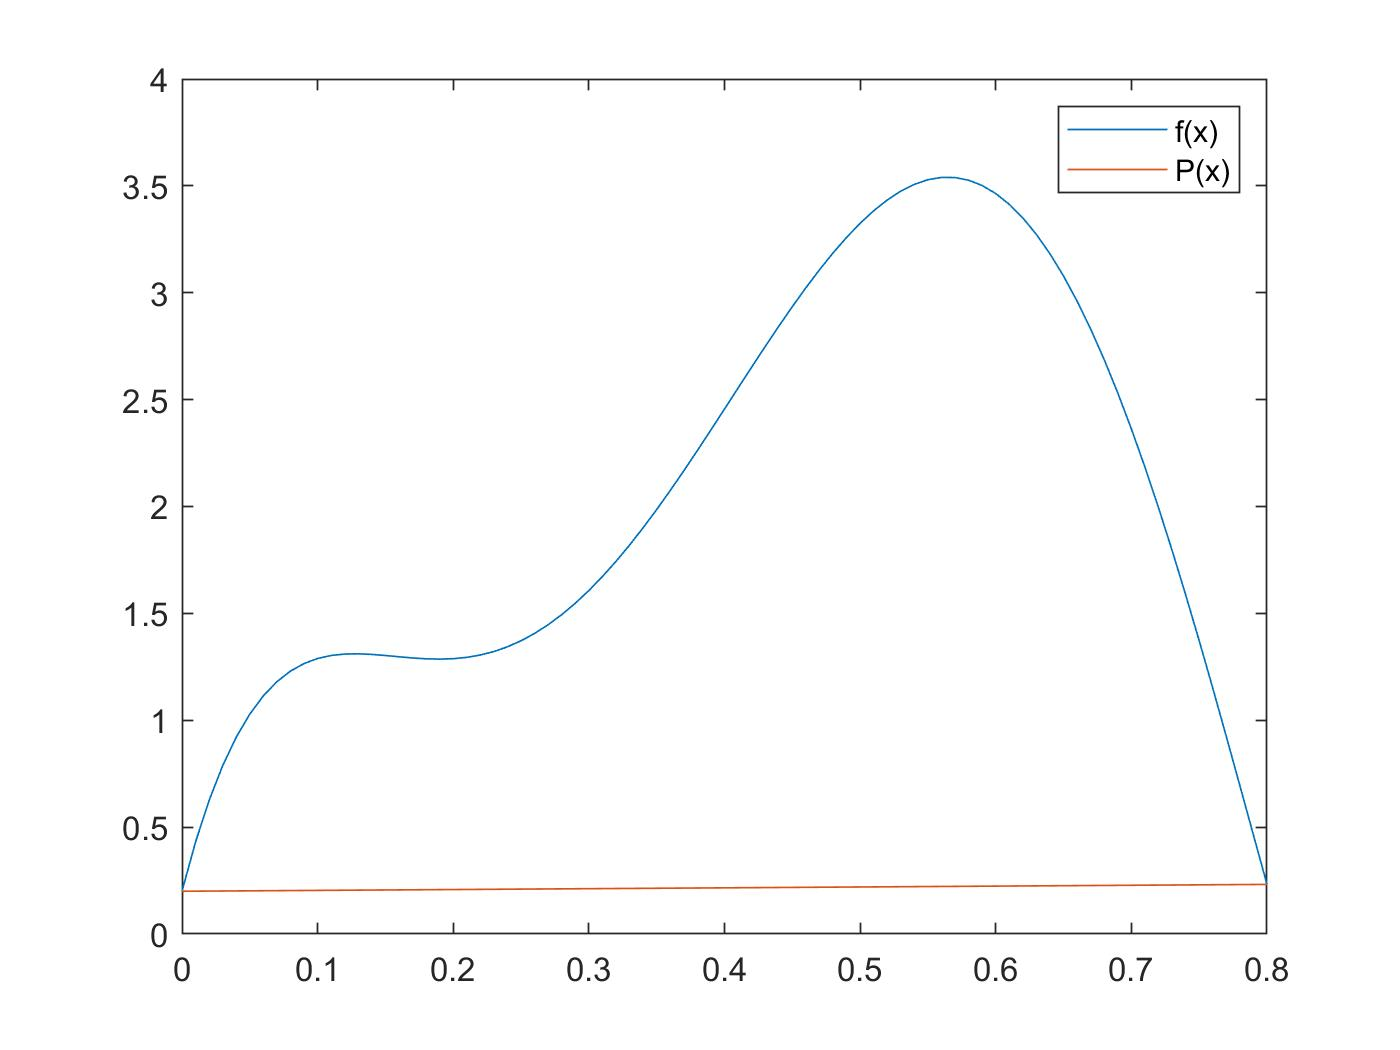
\includegraphics[scale=0.3]{lect15_ex1}
  \caption{Example 1 plot}
  \label{fig:lect15_ex1}
\end{figure}


\subsection{Newton-Cotes closed quadrature formulas - n=2} 

For the case $n=2$ the quadratic interpolating polynomial is: 

\[
P(x) = \frac{(x-x_1)(x-x_2)}{(x_0-x_1)(x_0-x_2)}f(x_0)
+ \frac{(x-x_0)(x-x_2)}{(x_1-x_0)(x_1-x_2)}f(x_1)
+ \frac{(x-x_0)(x-x_1)}{(x_2-x_0)(x_2-x_1)}f(x_2)
\]
\begin{figure} 
  \centering
  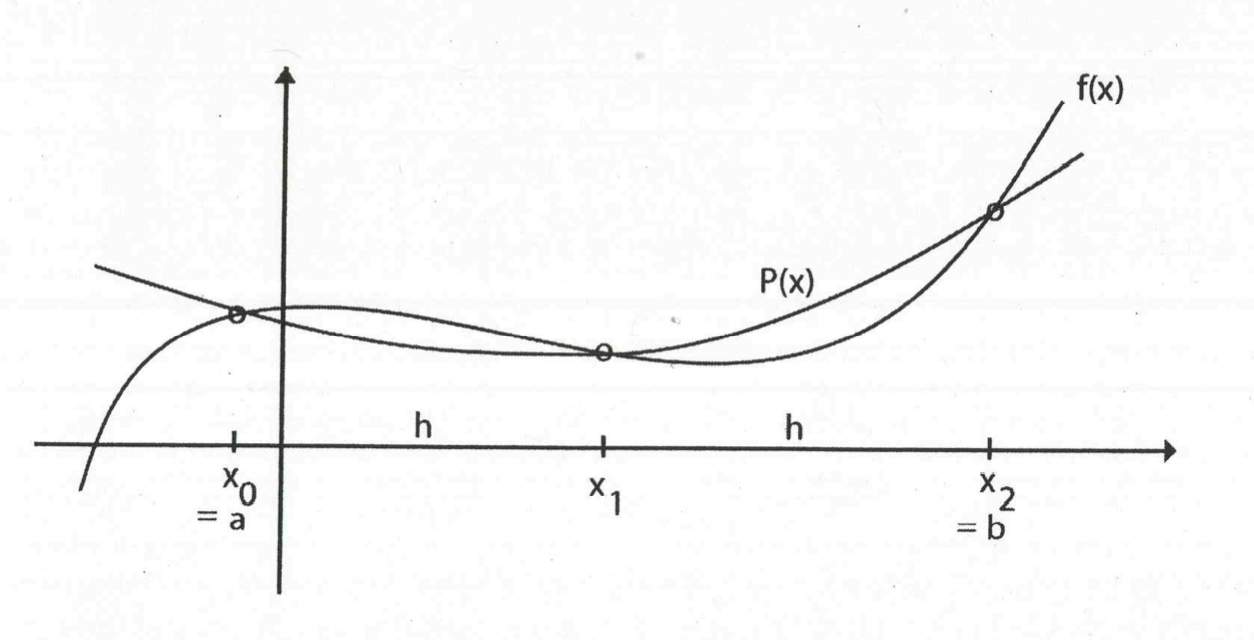
\includegraphics[scale=0.6]{quadratic_interpolating}
  \caption{Quadratic interpolating polynomial}
  \label{fig:linear}
\end{figure}




\noindent 
As in the case $n=1$, the quadrature formula for approximating $\int_a^{b} f(x)dx$ is obtained by integrating $P(x): \int_{a}^{b}f(x)dx \approx \int_{x_0}^{x_2}P(x)dx$. 

This gives: 
\[
   \int_{a}^{b} f(x)dx \approx \frac{h}{3}(f(x_0) + 4 f(x_1) + f(x_2))
\]
\noindent 
where now $h=\frac{b-a}{2}$. This is called {\bf Simpson's rule} or {\bf Simpson's 1/3 rule}, and its {\bf truncation error} is given by: 
\[
\int_{a}^{b}f(x)dx - \int_{x_0}^{x_2} P(x)dx = -\frac{h^5}{90} f^{(4)}(\xi), \mbox { for some } \xi \in [a,b] 
\]


\subsubsection{Example 2} 

Use the 1/3 Simpson's Rule to numerically integrate $f(x)=0.2+25x-200x^2+675x^3-900x^4+400x^5$ from $a=0$ to $b=0.8$. \\

{\bf Solution}
First, we need $f(0)$, $f(0.4)$ and $f(0.8)$ with $h=\frac{b-a}{2}=\frac{0.8}{2}=0.4$.

\[
f(0)=0.2
\]
\[
f(0.4)=0.2+25(0.4)-200(0.4)^2+675(0.4)^3-900(0.4)^4+400(0.4)^5 = 2.456
\]
\[
f(0.8)=0.2+25(0.8)-200(0.8)^2+675(0.8)^3-900(0.8)^4+400(0.8)^5 = 0.232
\]

So,

\[
\int_0^{0.8}f(x)dx \approx \frac{h}{3}[f(x_0)+4f(x_1)+f(x_2)] = \frac{0.4}{3}[0.2+4(2.456)+0.232] = 1.367467
\]

The actual value is $\int_0^{0.8}f(x)dx=1.640533$. That means that the true absolute error is $|E_t|=|1.640533-1.367467|=0.2730667$. In MATLAB,

\begin{verbatim}
>> x=0:0.01:0.8;
>> fx=0.2+25*x-200*x.^2+675*x.^3-900*x.^4+400*x.^5;
>> Px = 0.2 + 11.24*x - 14*x.^2;
>> plot(x,fx,x,Px)
>> legend('f(x)','P(x)')
\end{verbatim}

\begin{figure} 
  \centering
  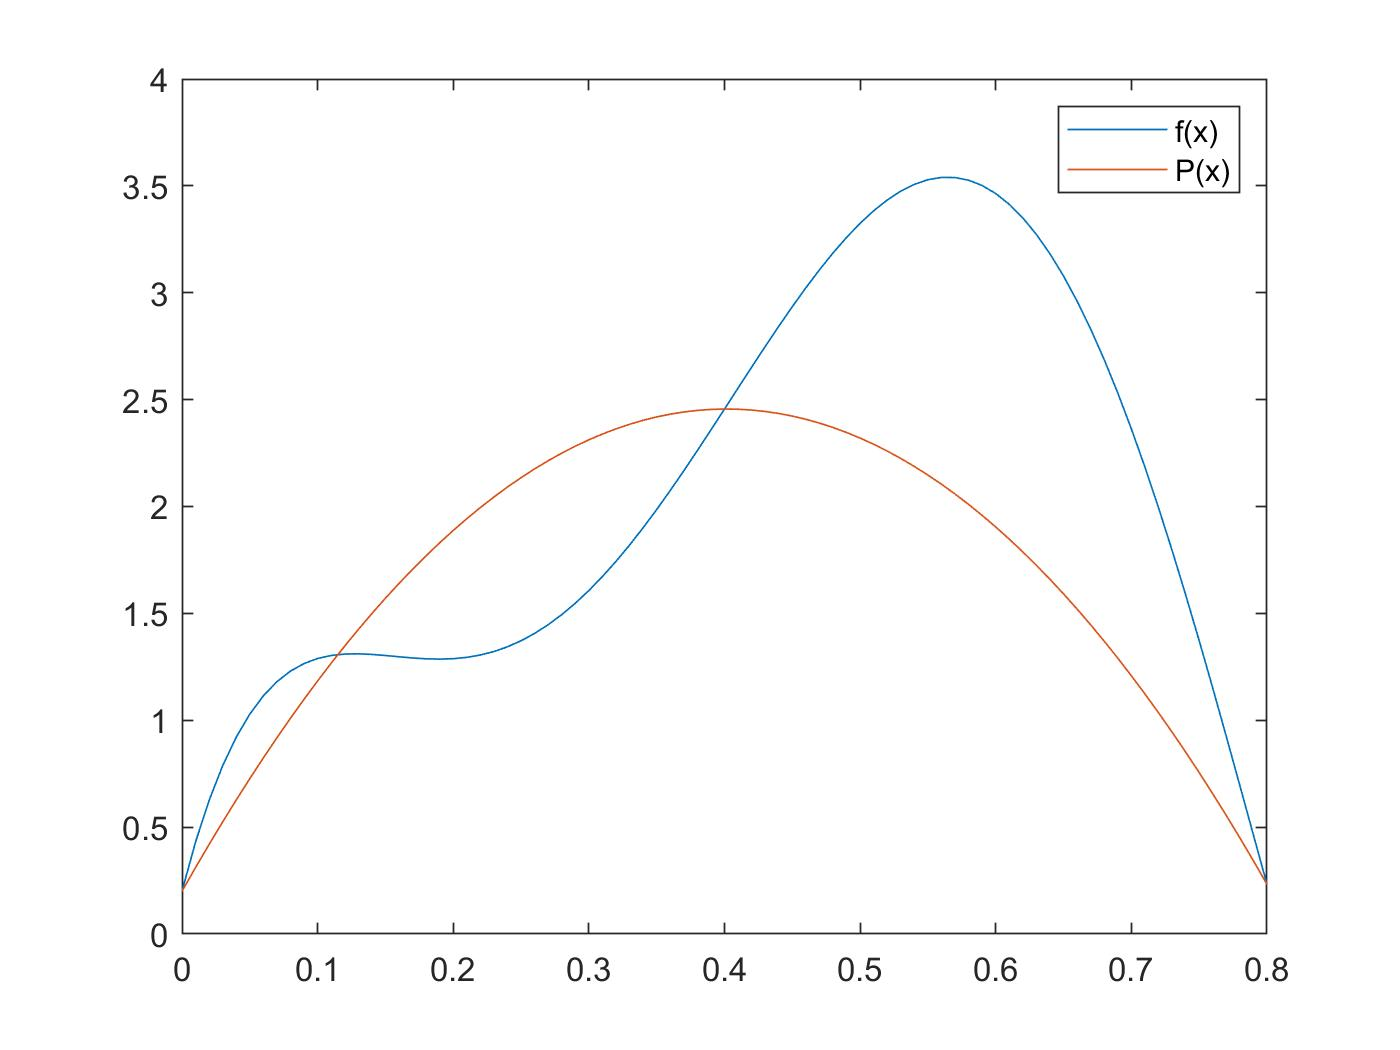
\includegraphics[scale=0.3]{lect15_ex2}
  \caption{Example 2 plot}
  \label{fig:lect15_ex2}
\end{figure}

\subsection{Quadrature formula for n=3} 

The Newton-Cotes closed quadrature formula for $n=3$, in which $f(x)$
is approximated by a cubic polynomial that interpolates at four
equally-spaced points, is:
\[
\int_{a}^{b} f(x)dx \approx \frac{3h}{8} (f(x_0) + 3 f(x_1) + 3 f(x_2) + f(x_3)), 
\mbox { where } h = \frac{b-a}{3}
\]

The truncation error for this is
\[
E_t=\frac{-3}{80}h^5f^{(4)}(\xi)
\]
\noindent
for some $\xi \in [a,b]$.

\subsubsection{Example 3} 

Use the 3/8 Simpson's Rule to numerically integrate $f(x)=0.2+25x-200x^2+675x^3-900x^4+400x^5$ from $a=0$ to $b=0.8$. \\

{\bf Solution}
First, we need $f(0)$, $f(0.8/3)$, $f(1.6/3)$ and $f(0.8)$ with $h=\frac{b-a}{2}=\frac{0.8}{3}$.

\begin{align*}
&f(0)=0.2 \\
&f(0.8/3)=0.2+25(0.8/3)-200(0.8/3)^2+675(0.8/3)^3-900(0.8/3)^4+400(0.8/3)^5 = 1.432724 \\
&f(1.6/3)=0.2+25(01.6/3)-200(1.6/3)^2+675(1.6/3)^3-900(1.6/3)^4+400(1.6/3)^5 = 3.487177 \\
&f(0.8)=0.2+25(0.8)-200(0.8)^2+675(0.8)^3-900(0.8)^4+400(0.8)^5 = 0.232
\end{align*}

So,

\begin{align*}
\int_0^{0.8}f(x)dx &\approx \frac{3h}{8}[f(x_0)+3f(x_1)+3f(x_2)+f(x_3)] \\
&= \frac{3(0.8/3)}{8}[0.2+3(1.432724)+3(3.487177)+0.232] = 1.5191703
\end{align*}

The actual value is $\int_0^{0.8}f(x)dx=1.640533$. That means that the true absolute error is $|E_t|=|1.640533-1.5191703|=0.1213630$. In MATLAB,

\begin{verbatim}
>> x=0:0.01:0.8;
>> fx=0.2+25*x-200*x.^2+675*x.^3-900*x.^4+400*x.^5;
>> Px = 0.2 - 4.5822*x + 48.8889*x.^2 - 53.8889*x.^3;
>> plot(x,fx,x,Px)
>> legend('f(x)','P(x)')
\end{verbatim}

\begin{figure} 
  \centering
  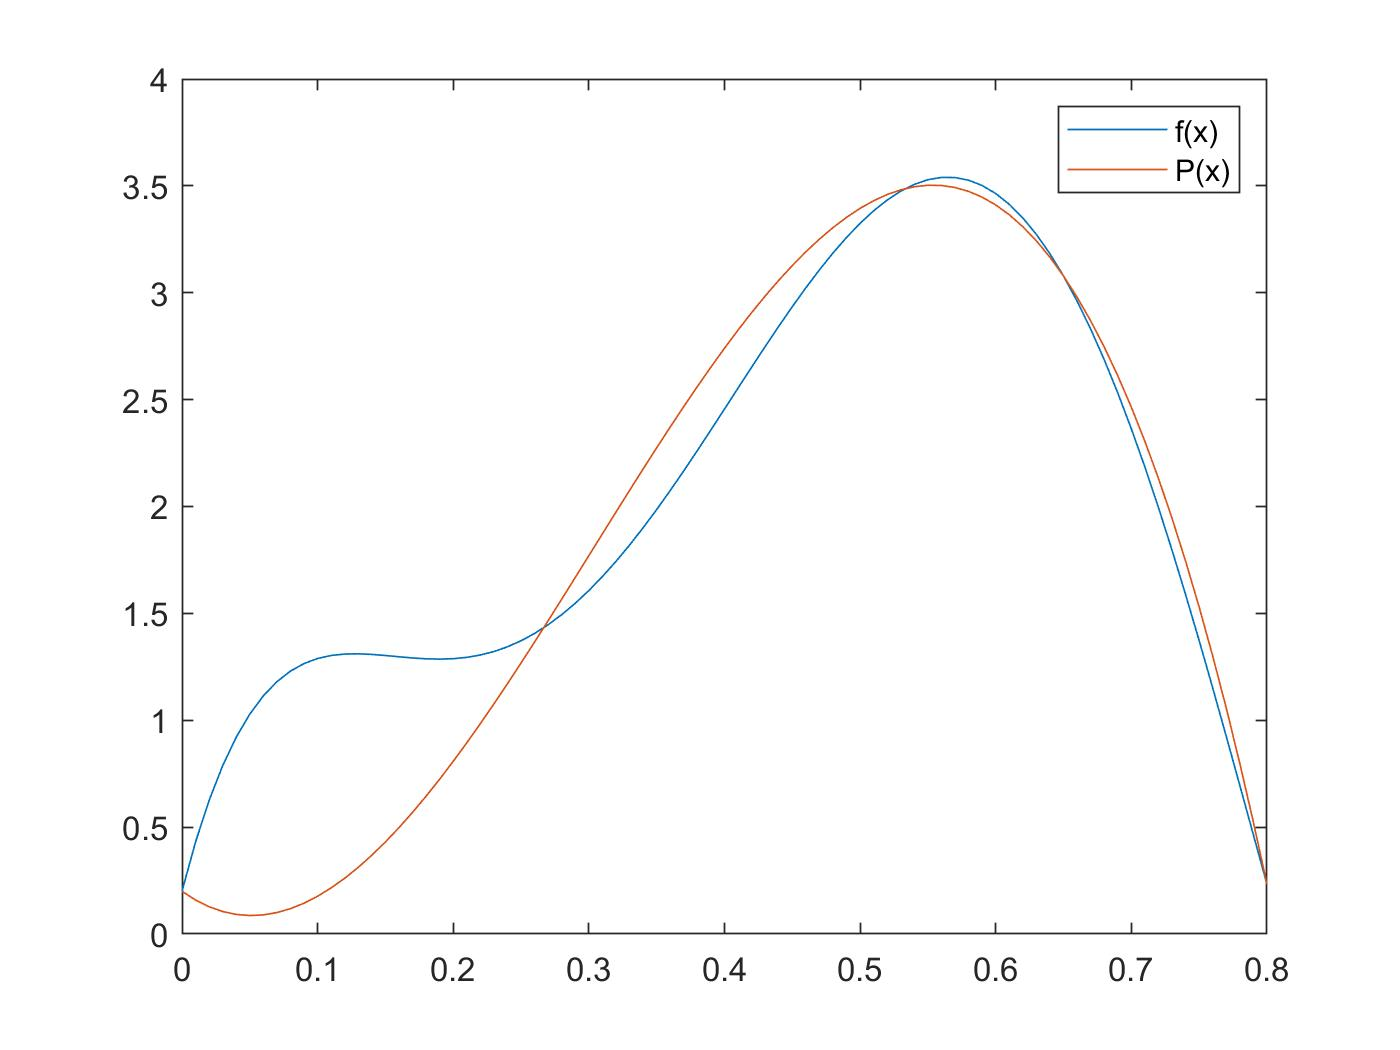
\includegraphics[scale=0.3]{lect15_ex3}
  \caption{Example 3 plot}
  \label{fig:lect15_ex3}
\end{figure}
\section{Composite Newton-Cotes Formulas} 

This section corresponds to sections 21.1.2, 21.2.2, 21.3, and 21.4 of the text.

{\bf Objective:} We want the {\bf truncation error $\rightarrow 0$} as the {\bf number of quadrature points $\rightarrow \infty$.}
Note: this does not happen in general as $n$, the order of the interpolating polynomial, $\rightarrow \infty$ (Runge phenomenon).
{\bf Solution:} We use composite (multiple-application) quadrature formulas.


\subsection{Trapezoidal rule} 

{\bf Main idea:} for $m \geq 1$, apply a closed N-C formula (with $n$ small) $m$ times on $[a,b]$. 

\noindent 
{\bf Example:} Trapezoidal rule $(n=1)$ 
\\
For any $m \geq 1$, let $h = \frac{b-a}{m}$, subdivide $[a,b]$ into $m$ subintervals of length $h$, and apply the trapezoidal rule on each subinterval. 


\begin{figure}[h] 
  \centering
  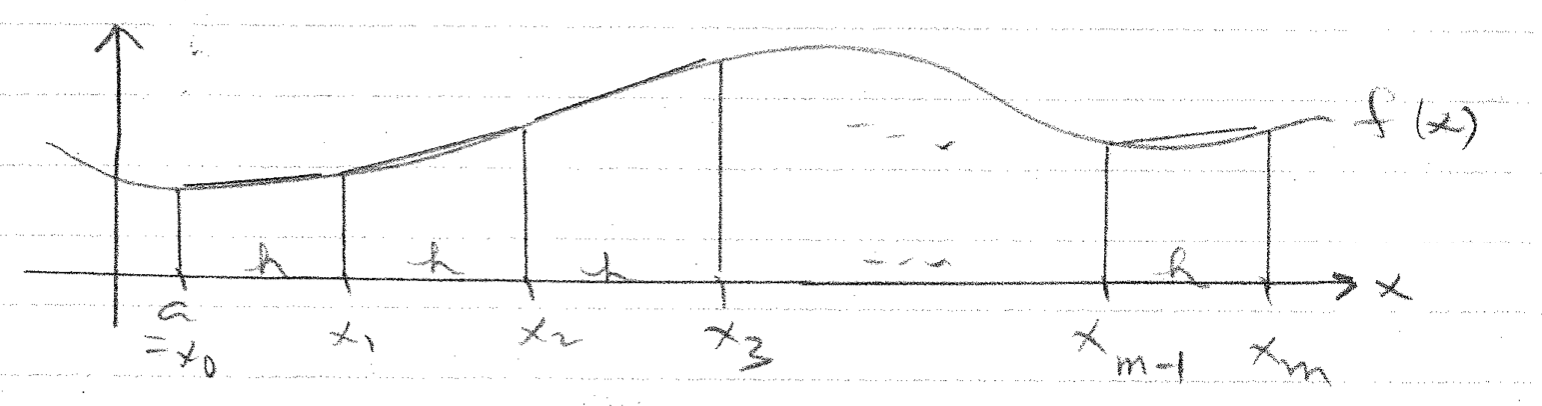
\includegraphics[scale=0.4]{composite_nc}
  \label{fig:composite_nc}
\end{figure}

{\bf Composite trapezoidal rule} 
\noindent
So, we apply the Trapezoidal rule $m$ times using the $m+1$ evenly spaced data points $(x_0,f(x_0))$, $(x_1,f(x_1))$, ..., $(x_m,f(x_m))$ where $a=x_0$ and $b=x_m$. That is, we linearly interpolate each of the subintervals and integrate usng the resulting interpolating polynoimal over each region.
\begin{align*} 
& \int_{a}^{b} f(x)dx = \int_{x_0}^{x_1}f(x)dx +  \int_{x_1}^{x_2}f(x)dx + \dots + \int_{x_{m-1}}^{x_m}f(x)dx \\ 
\approx & \int_{x_0}^{x_1}P_0(x)dx +  \int_{x_1}^{x_2}P_1(x)dx + \dots + \int_{x_{m-1}}^{x_m}P_{m-1}(x)dx \\
=& \frac{h}{2} \left [ f(x_0) + f(x_1) \right ] + \frac{h}{2} \left [ f(x_1) + f(x_2) \right ] + \dots + \frac{h}{2} \left [ f(x_{m-1}) + f(x_{m}) \right ] \\ 
=& \frac{h}{2} \left [ f(x_0) + 2\sum_{i=1}^{m-1} f(x_i) + f(x_m) \right ] 
\end{align*} 

This is called the composite trapezoial rule. 


{\bf Truncation Error}
\begin{align*} 
E_t =& -\frac{h^3}{12} f''(\xi_1) -\frac{h^3}{12} f''(\xi_2) - \dots - -\frac{h^3}{12} f''(\xi_m)  \\
=& -\frac{h^3}{12} \left [ f''(\xi_1) + f''(\xi_2) + \dots + f''(\xi_m) \right ] 
\end{align*} 
where $x_{i-1} \leq \xi_i \leq x_i$. 

We know that: 
\[
\min_{1 \leq i \leq m} f''(\xi_i) \leq \frac{f''(\xi_1) + f''(\xi_2) + \dots + f''(\xi_m)}{m} \leq \max_{1 \leq i \leq m} f''(\xi_i) 
\]

If $f''(x)$ is continuous on $[a,b]$, then there exists a value $\mu \in [a,b]$ such that: 

\[
f''(\mu) = \frac{f''(\xi_1) + f''(\xi_2) + \dots + f''(\xi_m)}{m} 
\]

This is called the intermediate value theorem. 

\[
E_t = - \frac{h^3}{12} [ m f''(\mu)] = - \frac{(b-a)}{12} h^2 f''(\mu) 
\]

since $h = \frac{b-a}{m}$. 

{\bf Important point} 

\[\lim_{m \rightarrow \infty} E_t = \lim_{h \rightarrow 0} E_t = 0
\]
provided that $f''(x)$ is continuous on $[a,b]$. 

\noindent 
(there is no comparable result as $n \rightarrow \infty$, where $n$ is the degree of the interpolating polynomial) 

\subsubsection{Example 1} Use the two-segment ($m=2$) trapezoidal rule to estimate the integral of $f(x)=0.2+25x-200x^2+675x^3-900x^4+400x^5$ from $a=0$ to $b=0.8$. Recall that the correct value for the integral is $\int_0^{0.8} f(x)dx=1.640533$. \\

\noindent
{\bf Solution} Here, we need three data points, $f(0)=0.2, f(0.4)=2.456$, and $f(0.8)=0.232$. Also, $h=\frac{b-a}{m}=\frac{0.8}{2}=0.4$. Thus,

\begin{align*}
\int_0^{0.8} f(x)dx &\approx \frac{h}{2} \left[f(x_0)+2f(x_1)+f(x_2) \right] \\
&= \frac{0.4}{2}\left[f(0)+2f(0.4)+f(0.8) \right] \\
&= 0.2\left[0.2+2(2.456)+0.232 \right] \\
&=1.0688
\end{align*}

\noindent
That means $|E_t| = |1.640533 - 1.0688| = 0.57173$.

\subsubsection{Implementation} Usual implementation of composite trapezoidal: 
\begin{itemize} 
\item Initialize $m=1$ 
\item Repeatedly double $m$ (m=1,2,4,8,16,32,\dots )
\item Until two consecutive approximations are sufficiently close 
\end{itemize} 


The reason for using these values of $m$ is that they permit re-use of the function evaluations from previous evaluations

 i.e all values $f(x_i)$ computed for $m=k$ can be re-used for $m=2k$. 


\begin{figure}[h] 
  \centering
  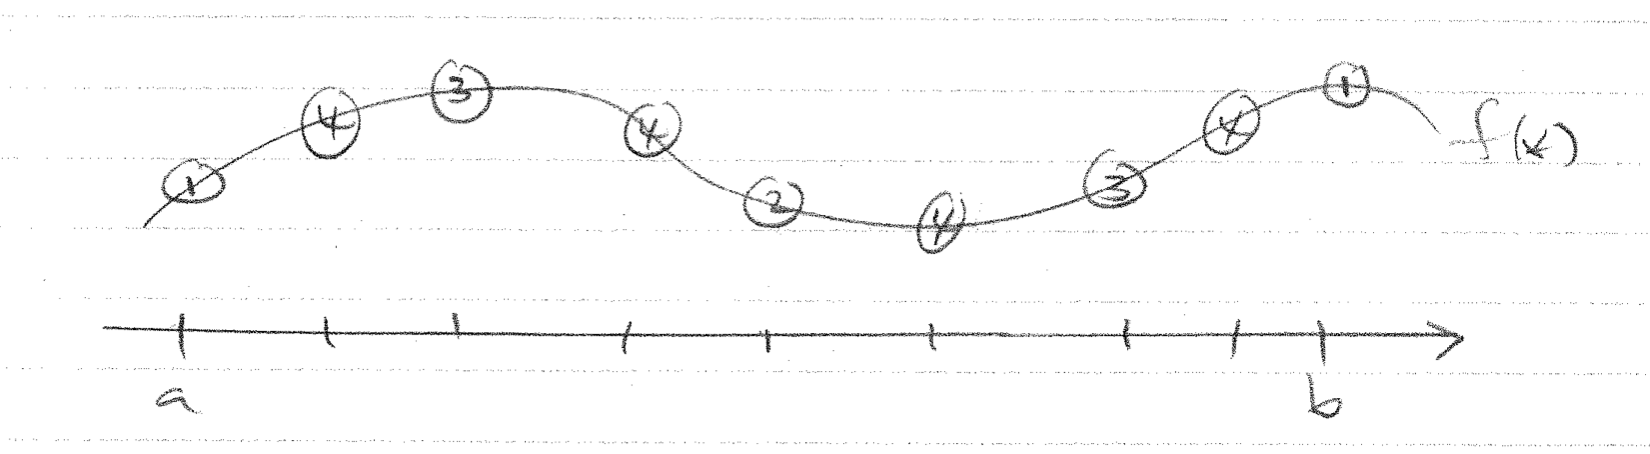
\includegraphics[scale=0.4]{reuse_of_points}
  \label{fig:reuse}
\end{figure}
 
\subsection{Composite Simpson's Rule}

Each application of Simpson's rule requires 2 subintervals on the interval of integration and 3 quadrature points. Thus, $m$ applications of Simpson's rule on $[a,b]$ require that $[a,b]$ be subdivided into $2m$ subintervals using $2m+1$ quadrature points. Each subinterval then is of length
\[
h=\frac{b-a}{2m}
\]

Thus, at the $jth$ subinterval we have the three quadrature points $x_{2j-2}$, $x_{2j-1}$, and $x_{2j}$, and
\[
\int_{x_{2j-2}}^{x_{2j}} f(x)dx \approx \frac{h}{3} \left [ f(x_{2j-2}) + 4f(x_{2j-1}) + f(x_{2j}) \right ] 
\]			     

When $m=1$ (regular Simpson's rule) we have $2(1)+1=3$ quadrature points and 2 subintervals each of length $h=\frac{b-a}{2}$.

When $m=2$, we apply Simpson's rule twice. We need $2(2)+1=5$ quadrature points to create $4$ subintervals each of length $h=\frac{b-a}{4}$.

\vspace{\baselineskip}
Here,
\begin{align*} 
& \int_{a}^{b} f(x)dx \\
& \approx \frac{h}{3} \left [ f(x_0) + 4f(x_1) + f(x_2) \right ] + \frac{h}{3} \left [ f(x_2) + 4f(x_3) + f(x_4) \right ] \\
& = \frac{h}{3} \left [ f(x_0) + 4f(x_1) + 2f(x_2) + 4f(x_3) + f(x_4) \right ]
\end{align*} 

In general, when $m \geq 1$, the composite Simpson's rule approximation is
\begin{multline*} 
 \int_{a}^{b} f(x)dx \\
 \approx \frac{h}{3}  [f(x_0) + 4f(x_1) + 2f(x_2) + 4f(x_3) + 2f(x_4) + \\ 
     \dotsm + 2f(x_{2m-2}) + 4f(x_{2m-1}) + f(x_{2m})]  \\
 = \frac{h}{3} \left [ f(x_0) + 4\sum_{j=1}^{m}f(x_{2j-1}) + 2\sum_{j=1}^{m-1}f(x_{2j}) + f(x_{2m}) \right ]
\end{multline*} 


{Truncation Error}
\begin{align*} 
E_t =& -\frac{h^5}{90} f^{(4)}(\xi_1) -\frac{h^5}{90} f^{(4)}(\xi_2) - \dots - -\frac{h^5}{90} f^{(4)}(\xi_m)  \\
=& -\frac{h^5}{90} \left [ f^{(4)}(\xi_1) + f^{(4)}(\xi_2) + \dots + f^{(4)}(\xi_m) \right ] \\
=& - \frac{h^5}{90} [ m f^{(4)}(\mu)]
\end{align*} 
where $a \leq \mu\leq b$ and $f^{(4)}(x)$ is continous. So,
\begin{align*} 
E_t = -\frac{(b-a)h^4}{180}f^{(4)}(\mu)
\end{align*} 
since $h = \frac{b-a}{2m}$. 

\subsubsection{Example 2} Use the two-segment ($m=2$) composite Simpson's rule to estimate the integral of $f(x)=0.2+25x-200x^2+675x^3-900x^4+400x^5$ from $a=0$ to $b=0.8$. Recall that the correct value for the integral is $\int_0^{0.8} f(x)dx=1.640533$. \\

\noindent
{\bf Solution} Here, we need  five data points, $f(0)=0.2, f(0.2)=1.288,f(0.4)=2.456,f(0.6)=3.464$, and $f(0.8)=0.232$. Also, $h=\frac{b-a}{2m}=\frac{0.8}{4}=0.2$. Thus,

\begin{align*}
\int_0^{0.8} f(x)dx &\approx \frac{h}{3} \left[f(x_0)+4f(x_1)+2f(x_2)+4f(x_3)+f(x_4) \right] \\
&= \frac{0.2}{3}\left[f(0)+4f(0.2)+2f(0.4)+4f(0.6)+f(0.8) \right] \\
&= \frac{0.2}{3}\left[0.2+4(1.288)+2(2.456)+4(3.464)+0.232 \right] \\
&=1.623467
\end{align*}

\noindent
That means $|E_t| = |1.640533 - 1.623467| = 0.017067$.

\end{document} 















